\documentclass[a4paper,12pt]{article}
\usepackage{mathtools,amsfonts,amssymb,amsmath, bm,commath,multicol}
\usepackage{algorithmicx, tkz-graph, algorithm, fancyhdr, pgfplots}
\usepackage{fancyvrb}

\usepackage[noend]{algpseudocode}

\pagestyle{fancy}
\fancyhf{}
\rhead{A. Casarico, N. Rao, I. Gogitidze, J. Westermann}
\lhead{15F020 Problemset 2}
\rfoot{\thepage}


\DefineVerbatimEnvironment{juliaout}{Verbatim}{}
\DefineVerbatimEnvironment{juliacode}{Verbatim}{fontshape=sl, fontsize=\tiny}
\DefineVerbatimEnvironment{juliaterm}{Verbatim}{}


\begin{document}




\section{Black-Scholes Model}
$$
dX_t = 2X_tdt + 1.5X_tdB_t \ \ \ \ \ \ \ X_0 = 1
$$
%
\subsection*{Solution}
Identifying this as a Block-Scholes model, we can write down the key parameters:
\begin{align*}
X_0 = 1 &= S_0 \\
a(t, x) = 2X_t &= \mu x \\
b(t, x) = 1.5X_t &= \sigma x
\end{align*}
%
Which we plug into the known Black-Scholes solution:
%
\begin{align*}
S_t &= e^{\sigma W_t + (\mu - \frac{\sigma^2}{2})t} \\
S_t &= e^{\frac{3}{2}W_t + \frac{7}{8}t}
\end{align*}
\subsection*{Simulations}
Here we plot simulations for increasing N, holding T fixed. As expected by the theory behind Euler's method, as N increases, and as the time increments decreas towards 0, the method becomes a better and better approximation of the true model.
\subsubsection*{Black Scholes Euler Simulation for N = 10, T = 1}
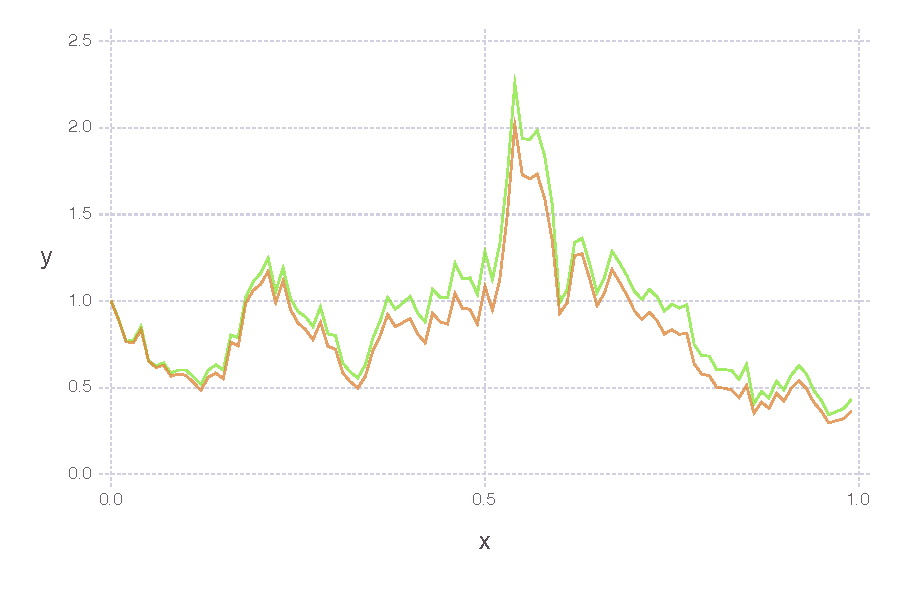
\includegraphics[width=\linewidth]{figures/problemset_2_1.pdf}



\subsubsection*{Black Scholes Euler Simulation for N = 50, T = 1}
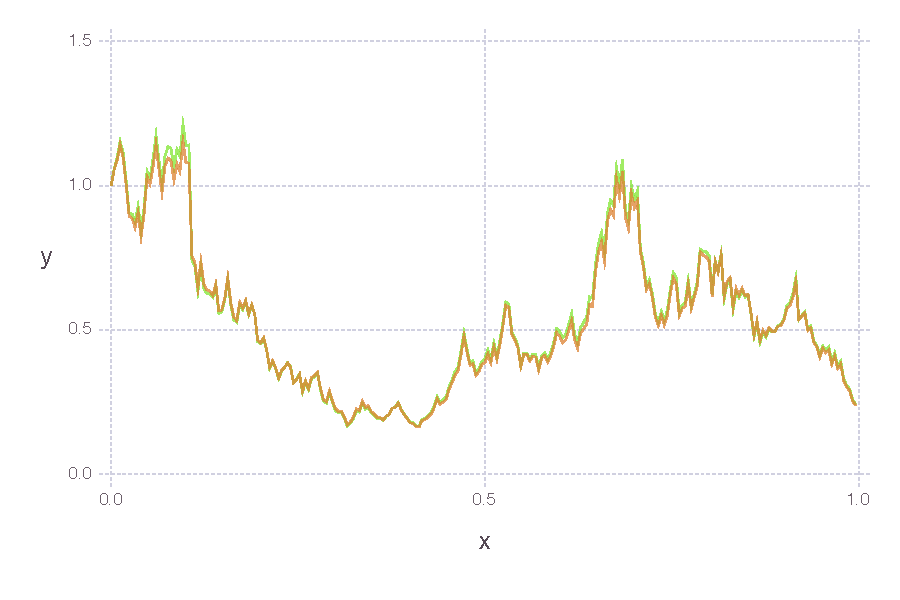
\includegraphics[width=\linewidth]{figures/problemset_3_1.pdf}



\subsubsection*{Black Scholes Euler Simulation for N = 1000, T = 1}
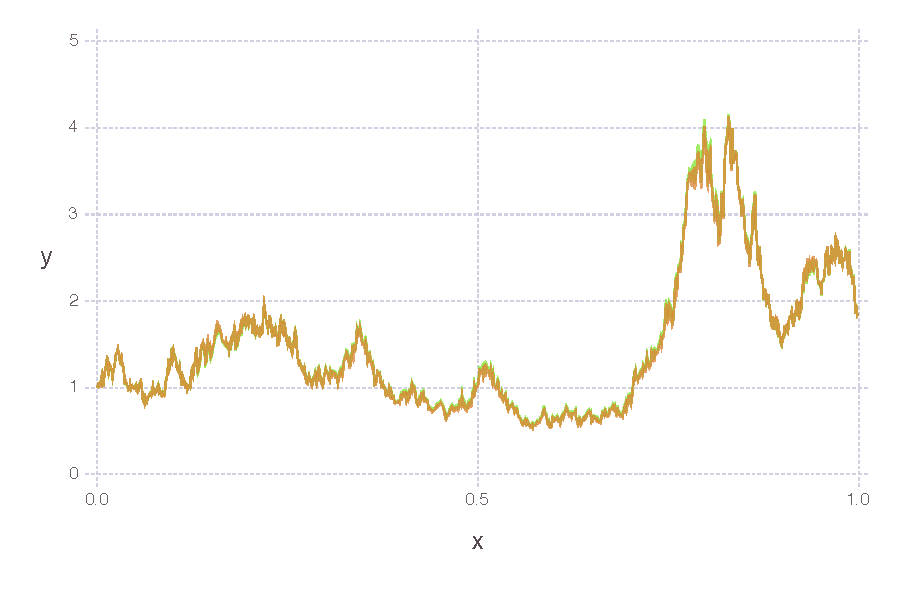
\includegraphics[width=\linewidth]{figures/problemset_4_1.pdf}


\section{Vasicek Model}
$$
dX_t = a(m - X_t)dt + \sigma dB_t \ \ \ \ \ \ \ X_0 = x
$$
%
\subsection{}
Differentiating the given equation, we find the solution to the Vasicek SDE:
\begin{align*}
Y_t &= e^{at}X_t \\
\frac{d}{dt}Y_t &= ae^{at}X_t + e^{at}\frac{dX_t}{dt} + \frac{1}{2}*0 \\
dY_t &= ae^{at}X_tdt + e^{at}dX_t \\
dY_t &= ae^{at}X_tdt + e^{at}( a(m - X_t)dt + \sigma dB_t) \\
dY_t &= ae^{at}X_tdt + ame^{at}dt - ae^{at}X_tdt + e^{at} \sigma dB_t \\
dY_t &= ame^{at}dt + e^{at} \sigma dB_t \\
\int_o^t dY_sds &= \int_0^t ame^{as}ds + \int_0^t e^{as} \sigma dB_s \\
Y_t - Y_o &= \frac{1}{a} ame^{at} - \frac{1}{a}ame^{a*0} + \int_0^t e^{as} \sigma dB_s \\
e^{at}X_t - X_0 &= me^{at} - me^{0} + \int_0^t e^{as} \sigma dB_s \\
X_t &= X_0e^{-at} + me^{at}e^{-at} - me^{-at} + e^{-at}\sigma \int_0^t e^{as} dB_s \\
X_t &= m - (X_0 - m)e^{-at} + e^{-at}\sigma \int_0^t e^{as} dB_s \\
\end{align*}

\subsection{}

\subsubsection*{Expectation of $X_t$}
\begin{align*}
\mathbb{E}[X_t] &= \mathbb{E} \bigg[ m - (X_0 - m)e^{-at} + e^{-at}\sigma \int_0^t e^{as} dB_s \bigg] \\
\mathbb{E}[X_t] &= m - (X_0 - m) e^{-at} + e^{-at}\sigma \mathbb{E} \bigg[ \int_0^t   e^{as} dB_s \bigg]
\end{align*}
%
By definition of brownian motion, $\int_0^t   e^{as} dB_s$ is a centered gaussian random variable, and therfore the expectation is 0 (as every increment of brownian motion has, of course, an expectation of 0). This leaves us with:
$$
\mathbb{E}[X_t] = m - (X_0 - m) e^{-at}
$$
%
\subsubsection*{Variance of $X_t$}
\begin{align*}
\text{Var}[X_t] &= \mathbb{E}[X_t^2] - \mathbb{E}[X_t]^2 \\
\text{Var}[X_t] &= \mathbb{E}[\big( m - (X_0 - m) e^{-at} \big)^2 + 2[...] + e^{-2at}\sigma^2 \int_0^t e^{as}dB_s ] -  \big( m - (X_0 - m) e^{-at} \big)^2 \\
\text{Var}[X_t] &= \big( m - (X_0 - m) e^{-at} \big)^2 + \mathbb{E}[ 2[...] + e^{-2at}\sigma^2 \int_0^t e^{as}dB_s ] -  \big( m - (X_0 - m) e^{-at} \big)^2 \\
\text{Var}[X_t] &=  \mathbb{E}[ 2e^{-at}\sigma\int_0^te^{as}dB_s(m - (X_0 - m)e^{-at})] + \mathbb{E} [ e^{-2at}\sigma^2 \big( \int_0^t e^{as}dB_s\big)^2 ] \\
\text{Var}[X_t] &=  e^{-2at}\sigma^2 \mathbb{E} [\big( \int_0^t e^{as}dB_s\big)^2 ] \\
\text{Var}[X_t] &=  e^{-2at}\sigma^2 \int_0^t \mathbb{E} [e^{2as}]ds \\
\text{Var}[X_t] &=  e^{-2at}\sigma^2 \int_0^t e^{2as}ds \\
\text{Var}[X_t] &=  e^{-2at}\sigma^2 (\frac{1}{2a}e^{2at} - \frac{1}{2a}e^{0}) \\
\text{Var}[X_t] &=  \frac{\sigma^2}{2a}(1 - e^{-2at})
\end{align*}

\subsubsection*{In the Limit}
Taking $ t \rightarrow \infty$ we see that:
\begin{align*}
\lim_{t \rightarrow \infty} \mathbb{E}[X_t] &= \lim_{t \rightarrow \infty} m - (X_0 - m) e^{-at} \\
\lim_{t \rightarrow \infty} \mathbb{E}[X_t] &= m - 0 \\
\lim_{t \rightarrow \infty} \mathbb{E}[X_t] &= m
\end{align*}
The expectation converges to the mean, which explains the mean-reverting phenomenon. Further, we can see the variance at the limit:
\begin{align*}
\lim_{t \rightarrow \infty} \text{Var}[X_t] &=  \lim_{t \rightarrow \infty} \frac{\sigma^2}{2a}(1 - e^{-2at}) \\
\lim_{t \rightarrow \infty} \text{Var}[X_t] &=  \frac{\sigma^2}{2a}(1 - 0) \\
\lim_{t \rightarrow \infty} \text{Var}[X_t] &=  \frac{\sigma^2}{2a}
\end{align*}
%
Which shows that at the limit, we expect the interest rates to converge to the mean, with a variance defined by the interaction between the variance of the underlying stochastic process and parameter a, which, as seen in the simulations, can be described as the speed or strength of the mean reversion. In the realm of interest rates, this tendency for mean reversion describes the theory that actual rates will always revert to the true rate of interest, despite temporary shocks.
%
\subsection{}
We plot several versions of the simulation to see the interaction of the parameters and the mean reversion. We make the mean 0 (the $\mu$ parameter), and make the initial value 5 for all simulations, which helps show the mean reversion (we expect the model to move, more-or-less swiftly depending on parameters, towards 0 from its initial point). As predicted, if $\sigma$ is large relative to a, the mean-reversion is undetectable, but if a is large compared to $\sigma$, the mean reversion becomes extremely clear.

\subsubsection{Vasicek Eueler simulation for $\sigma$ = 1, a = 5}
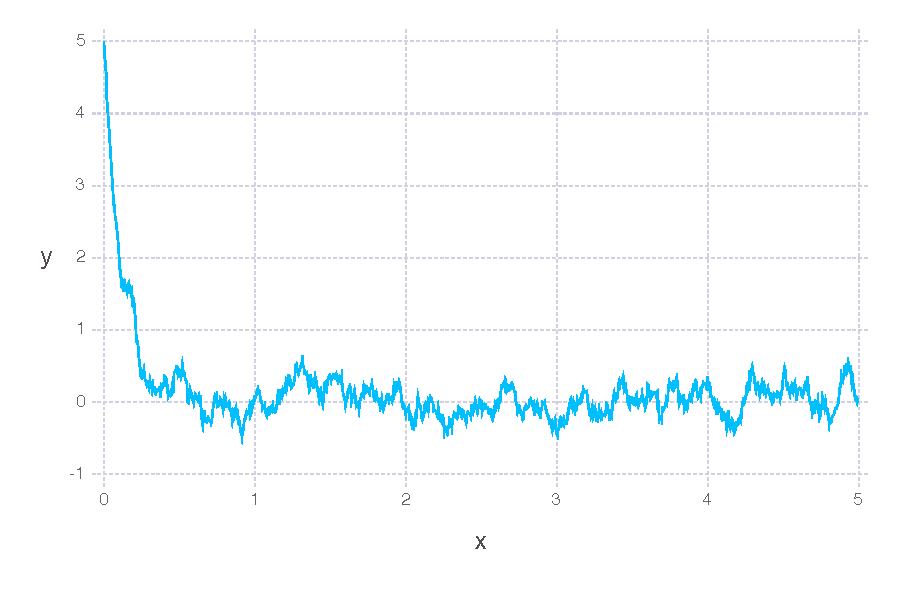
\includegraphics[width=\linewidth]{figures/problemset_5_1.pdf}



\subsubsection{Vasicek Eueler simulation for $\sigma$ = 2, a = 0.2}
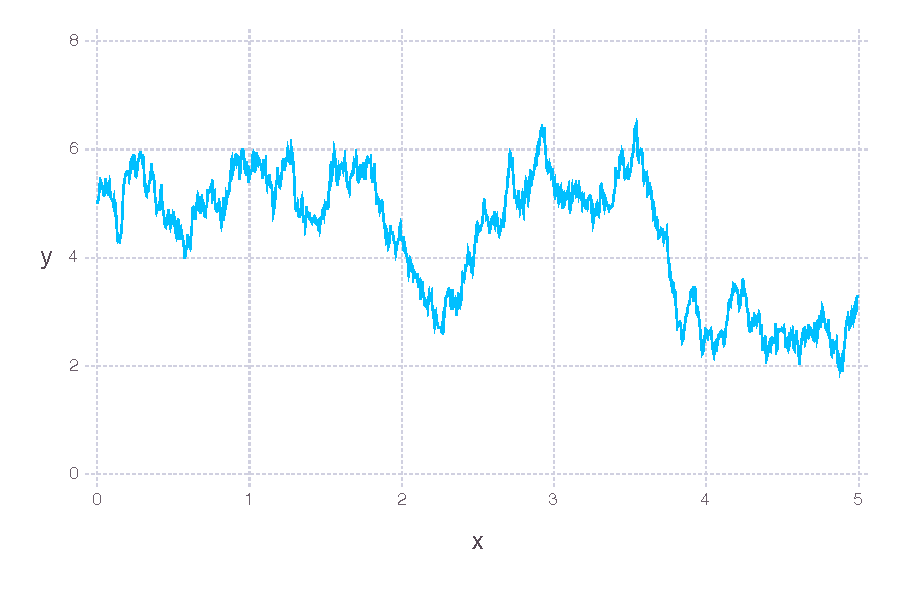
\includegraphics[width=\linewidth]{figures/problemset_6_1.pdf}



\subsubsection{Vasicek Eueler simulation for $\sigma$ = 10, a = 100}
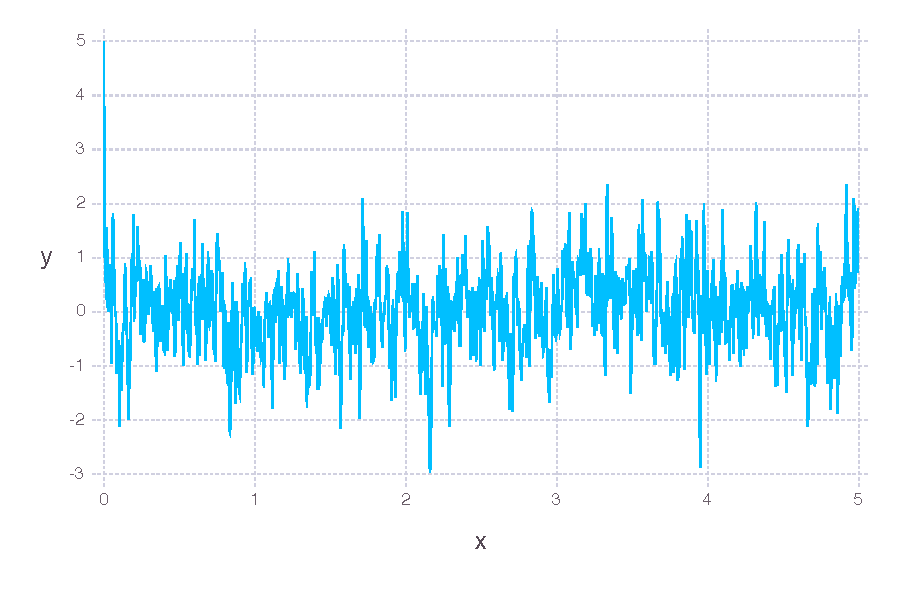
\includegraphics[width=\linewidth]{figures/problemset_7_1.pdf}



\section{Cox-Ingersoll-Ross Model}
$$
dr_t = (\alpha - \beta r_t)dt + \sigma \sqrt{r_t}dB_t \ \ \ \ \ \ \ r_0 = 0
$$

\subsection{}
Re-writing the differential equation:
$$
dr_t = \beta(\frac{\alpha}{\beta} - r_t)dt + \sigma \sqrt{r_t}dB_t
$$
Apply Ito's formula we get:
%
\begin{align*}
r_t &= \frac{\alpha}{\beta} + (r_0 - \frac{\alpha}{\beta})e^{- \beta t} + \sigma e^{- \beta t} \int_0^t e^{\beta s} \sqrt{r_s} dB_s \\
r_t &= \frac{\alpha}{\beta} - \frac{\alpha}{\beta}e^{- \beta t} + \sigma e^{- \beta t} \int_0^t e^{\beta s} \sqrt{r_s} dB_s \\
r_t &= \frac{\alpha}{\beta}(1 - e^{- \beta t}) + \sigma e^{- \beta t} \int_0^t e^{\beta s} \sqrt{r_s} dB_s
\end{align*}
%
Computing the expectation gives us:
\begin{align*}
\mathbb{E}[r_t] &= \mathbb{E} \bigg[ \frac{\alpha}{\beta}(1 - e^{-\beta t}) + \sigma e^{-\beta t} \int_0^te^{\beta s}\sqrt{r_s}dB_s \bigg] \\
\mathbb{E}[r_t] &= \frac{\alpha}{\beta}(1 - e^{-\beta t}) + \sigma e^{-\beta t} \ \mathbb{E} \bigg[ \int_0^te^{\beta s}\sqrt{r_s}dB_s \bigg] \\
\mathbb{E}[r_t] &= \frac{\alpha}{\beta}(1 - e^{-\beta t}) + \sigma e^{-\beta t} (0) \\
\mathbb{E}[r_t] &= \frac{\alpha}{\beta}(1 - e^{-\beta t}) \\
\end{align*}
Which, when taken to the limit, shows a mean reversion phenomenon, with the mean reverting to the ratio $\frac{\alpha}{\beta}$, which is in line with what we see in the simulations.
\begin{align*}
\lim_{t \rightarrow \infty} \mathbb{E}[r_t] &=  \lim_{t \rightarrow \infty} \frac{\alpha}{\beta}(1 - e^{-\beta t}) \\
\lim_{t \rightarrow \infty} \mathbb{E}[r_t] &=  \frac{\alpha}{\beta}(1 - 0) \\
\lim_{t \rightarrow \infty} \mathbb{E}[r_t] &=  \frac{\alpha}{\beta} \\
\end{align*}
%


\subsection{}
Simular to the Vasicek model, the CIR model for interest rates also exhibits a strong tendency for mean reversion, although here the mean is $\frac{\alpha}{\beta}$. Two trajectories suffices to show the relationship between $alpha$ and $\sigma$, holding the ratio $\frac{\alpha}{\beta}$ constant at .04, we simulate $\sigma = .05$ with differing parameters of $\alpha$ and $\beta$. Simular to the a parameter in the Vasicek model, here the size of $\alpha$ and $\beta$, holding their ratio constant, increases the strength/speed of the mean-reversion.

\subsubsection{CIR Eueler simulation for $\sigma$ = .05, $\alpha$ = .04, $\beta$ = 1}
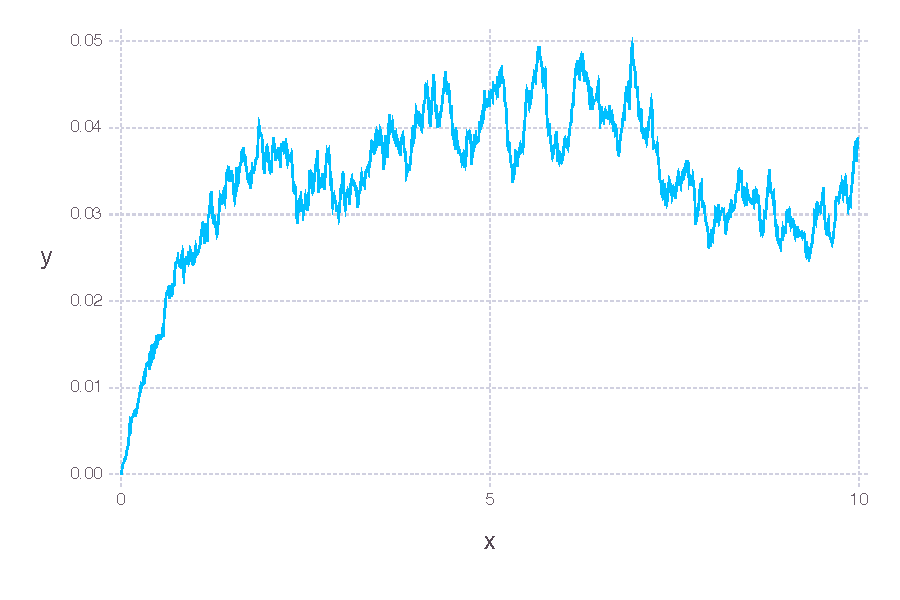
\includegraphics[width=\linewidth]{figures/problemset_8_1.pdf}



\subsubsection{CIR Eueler simulation for $\sigma$ = .05, $\alpha$ = 4, $\beta$ = 100}
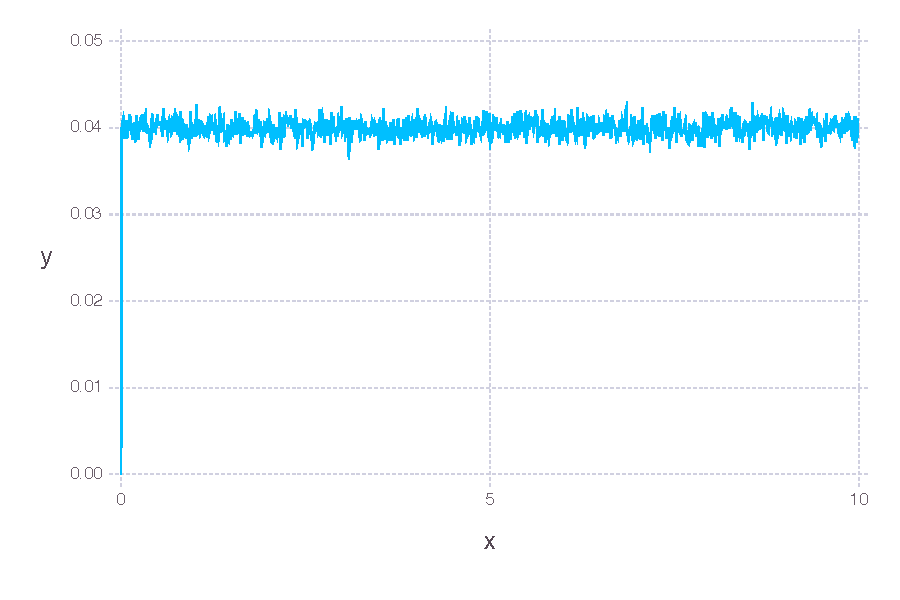
\includegraphics[width=\linewidth]{figures/problemset_9_1.pdf}




\section*{Code}
\begin{juliacode}
using Distributions
using DataFrames
using Gadfly
using Base.Test


#######################################
# Basic Brownian Motion Functions
#######################################
function make_walk(steps::AbstractArray{Float64,1}, start = 0.0)
    reduce((a,b) -> append!(a, a[end] + b), [start], steps)
end

make_time(N, T) = range(0, T/N, N)
brownian(N, T, start = 0.0) = make_walk(rand(Normal(0, sqrt(T/N)), N-1), start)

# Helper to cover the normal distributions from a brownian motion
function get_steps(B, N)
    step_size = Int(length(B)/N)
    steps = [B[i] - B[i-step_size] for i in (step_size + 1):step_size:length(B)]
end

@testset "get_steps" begin
    @test get_steps([0,2,4,6,8,10,12,14,16,18], 10) == fill(2, 9)
    @test get_steps([0,2,4,6], 4) == [2,2,2]
    @test get_steps([0,2,4,6,8,10,12,14,16,18], 5) == fill(4, 4)
end

geom(w, mu, sigma, t) = exp(sigma*w + (mu - sigma^2/2)*t)
geometric(brownian, time, mu, sigma) = [geom(b,mu,sigma,t) for (b,t) in zip(brownian, time)]

#######################################
# Eulers Method
#######################################

function eulers_method(B, N, T, a_fn, b_fn, start = 1.0)
    d = T/N
    W = get_steps(B, N)
    fn(x,w,t) = x + a_fn(t, x)*d + b_fn(t, x)*w
    reduce((a,i) -> append!(a, fn(a[end], W[i], i)), [start], 1:length(W))
    # extra = (length(B) - 1) % step_size
    # append!(base, fill(base[end], extra))
end

function geometric_euler(B, N, T, mu, sigma, start)
    a_fn(t, x) = mu*x
    b_fn(t, x) = sigma*x
    eulers_method(B, N, T, a_fn, b_fn, start)
end

#######################################
# Simulations
#######################################

function brownian_df(N, T, mu, sigma, start, B_N)
    B = brownian(B_N, T)
    path_time = make_time(B_N, T)
    path = DataFrame(value = geometric(B, path_time, mu, sigma),
                     time = path_time,
                     variable = fill("Brownian Path", B_N))
    euler_time = make_time(N, T)
    euler = DataFrame(value = geometric_euler(B, N, T, mu, sigma, start),
                      time = euler_time,
                      variable = fill("Euler Approximation", N))
    [path; euler]
end

function plot_bs(N, T, mu = 2, sigma = 1.5, start = 1.0, B_N = 1000)
    d = brownian_df(N, T, mu, sigma, start, B_N)
    plot(d, x = "time", y = "value", color = "variable", Geom.line)
end

function plot_vasicek(N, T, mu, sigma, a, start = 1.0)
    B = brownian(N, T)
    a_fn(t, x) = a*(mu - x)
    b_fn(t, x) = sigma
    euler = eulers_method(B, N, T, a_fn, b_fn, start)
    plot(x = make_time(N, T), y = euler, Geom.line)
end

function plot_cir(N, T, sigma, alpha, beta, start = 0.0)
    B = brownian(N, T)
    a_fn(t, r) = alpha - beta*r
    b_fn(t, r) = sigma*sqrt(r)
    euler = eulers_method(B, N, T, a_fn, b_fn, start)
    plot(x = make_time(N, T), y = euler, Geom.line)
end
\end{juliacode}


\end{document}